\chapter{Design}\label{chap:3}


This chapter undergoes the design steps that are taken in each stage of the research. Initially, this research is started as\textbf{ Compile time server architectures for Ballerina}. After analyzing the results of the initial set of experiments, the focus area is narrowed down to finding optimal thread pool size for different programming features. A machine learning approach is used to predict the thread pool size for a given set of programming features. Research questions remain unchanged from the beginning since thread pools are a crucial part of web server architectures and it is a tuning parameter for further improving the performance of server architecture. Literature review indicates that the performance of single web server architecture differs according to the type of operations it executes. Type of the operations can be extracted by analyzing the source code.  In simple terms, different web server architectures perform differently for different types of programs. Then based on the results further improvements and fine-tuning to the architecture are carried out in order to identify what parameters are required to change for maximizing the performance for each type of program. 

Formal research methodology is based on Design science research approach \cite{design_science}. Design science research approach requires the creation of an innovative, purposeful artifact for a special problem domain. The artifact must be evaluated in order to ensure its utility for the specified problem. In order to form a novel research contribution, the artifact must either solve a problem that has not yet been solved, or provide a more effective solution. Both the construction and evaluation of the artifact must be done rigorously, and the results of the research presented effectively both to technology-oriented and management-oriented audiences.


\begin{comment}
	This research tries to provide more effective solutions to a current problem and creates innovative solutions by introducing techniques to predict optimal thread pool size based on program features.
\end{comment}


The design of the research is divided into four stages. First off, existing Ballerina server architecture is carefully analyzed and designed how new architectures can be derived from it. New architectures are implemented by modifying the source code. Secondly, identified parameters from the first phase are tuned in order to maximize the performance in server architectures. In this phase, the size of the thread pool is tuned. Thirdly, differentiating the IO intensive features in the program and machine learning model is designed to predict the size of the thread pool. Afterward, \acrshort{AST} is parsed for extracting the identified features to feed into the machine learning model which is designed. 

This research consists of the following areas. The below sections span the design steps considered answering the research questions mentioned in the section.

Before diving into the design steps, it is important to specify the internal architecture of Ballerina run time. The next section briefly explains the internals of the Ballerina.



\section{Ballerina}\label{Sec_Ballerina}

This section provides an overview of current Ballerina architecture and explanation on how this research expects to use network awareness features in Ballerina language.  

In Ballerina connector calls that basically perform IO operations are explicitly presented in the source code as “ - $>$“. \acrfull{AST} parser extracts this information from the source to identify whether this call is a connector call and type of the connector call (HTTP, Database etc.).

Following is one example how the database calls are represented in ballerina code, note the -$>$ symbol.\\

\textit{stream$<$record{}, error$>$ resultStream = mysqlClient4 - $>$ query(<@untainted>query);}\\

Algorithm used for this operation is presented in section \ref{phase_iv}


\subsection{Ballerina internal architecture}

This section explains the main components of Ballerina run time.

\subsubsection{Netty Layer}

This layer is implemented using a library called Netty \cite{netty}. The primary task of the Netty layer is to listen for HTTP client connections and manage the session. It has its own thread pools to handle those connections. In original ballerina architecture, this layer simply handed over the incoming connection to the ballerina scheduler. Then the scheduler invokes relevant tasks for the client and returns the results to the Netty layer again for submitting back to the client. Inside the Netty layer, there are two types of threads. (1) \textbf{Boss threads} — Each bonded port has its own boss thread. For example, if the server listens on ports 80 and 443, then there are two boss threads. Main function of these threads is accepting the client requests. (2) \textbf{Worker threads} — Boss thread passes the accepted request to the worker thread. Worker threads then carries out the execution of the task. In Ballerina, these worker threads pass the request to the Ballerina scheduler.

\subsubsection{Scheduler}

Ballerina scheduler is the main component for every program/operation which executes. The Ballerina scheduler executes the client request using its own thread pool. The default thread pool size is two times the available processor count of the operating system. All the tasks which need to be executed are held in a queue. Then threads in the pool access the queue and execute the task. This is where major turnings are happening at the final stage of the research. 

\subsubsection{Resource function}

In Ballerina each API endpoint can be implemented as a resource function. That function includes all the implementation required to fulfill the task that the client is requested. More details about resource function are stated in chapter \ref{chap:4}. In this research, each resource function is considered a program.


Figure \ref{bal_internal} shows high level view of Ballerina architecture.

\begin{figure}[htbp]
	\begin{center}
		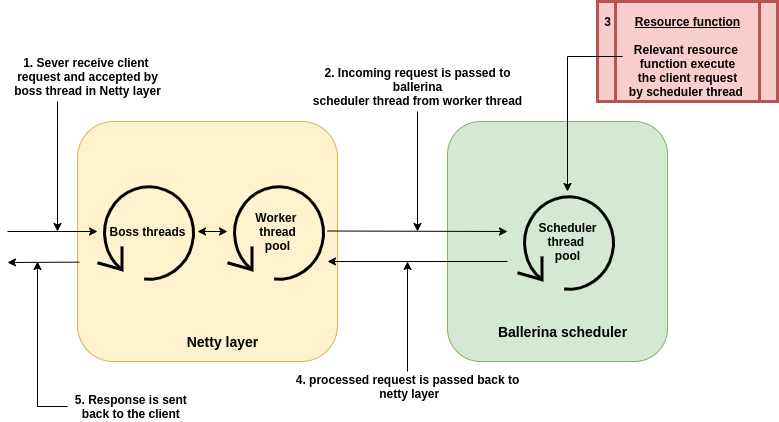
\includegraphics[scale=0.5]{figures/bal-internal.png}
	\end{center}
	\caption{Ballerina's internal architecture}
	\label{bal_internal}
\end{figure}

\section{Design steps}

The initial idea is coupled with the bound type of the program (CPU bound and IO-bound). Objectives were, (1) for a given Ballerina program identify its bound type, then (2) switch the server architecture which best suits the bound type. To determine the best server architecture, experiments are conducted. Following steps are taken to conduct the experiments. The below process is iterative.

\begin{itemize}
	\item Implement server architectures
	\item Use existing benchmark programs and implement new programs as necessary which have CPU intensive task and IO intensive tasks.
	\item Examine results.
	\item Debug and fine tune architectures based on results.
\end{itemize} 

\subsection{Testing process}

Each testing program is hosted as HTTP endpoints. Calling that endpoint invokes the relevant program. Jmeter act as a HTTP client. A typical web server is able to process concurrent HTTP requests. Jmeter can be configured to model this behavior. Jmeter continuously calls the given endpoint for a certain period under given configurations such as concurrency level. Then the following metrics are recorded,

\begin{itemize}
	\item Average latency — client HTTP requests are continuously sent to the web server and measure response time of each request. Then average is calculated.
	\item Standard deviation of latency — Standard deviation of above latency results.
	\item Throughput — Number of successful responses received per second.
	\item Error rate - Number of erroneous request as percentage of all request sent.
	\item Median, 75th percentile, 99th percentile of latency results.
\end{itemize} 

Then the performance is evaluated using above metrics. As an example when average latency is low and throughput is high for a given endpoint, that architecture's performance is good relative to others.
  

\begin{figure}[htbp]
	\begin{center}
		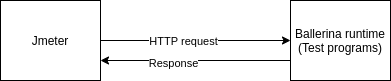
\includegraphics[scale=0.5]{figures/jmeter_bal.png}
	\end{center}
	\caption{Jmeter and Ballerina run time}
	\label{jmeter_testing}
\end{figure}



\subsection{Phase I - Implement and evaluate performance of different server architectures}

In this phase following server architectures are implemented. 

 \begin{itemize}
 	\item Original Ballerina architecture
 	\item Netty OIO
 	\item Removed Ballerina scheduler thread pool
 	\item Changing Ballerina scheduler thread pool size
 \end{itemize} 

The goal of implementing Netty OIO is to have a similar architecture of the thread per connection model. In this Netty's worker thread pool is configured to spawn a new thread per each client request. These threads block the execution until the task is finished. However, the Ballerina scheduler continues the execution in non-blocking fashion.

The expectation of removing the Ballerina scheduler is to inspect the behavior and performance when one thread pool is removed. The Netty layer's worker thread will carry out the execution of client tasks instead of the Ballerina scheduler thread. When there are multiple thread pools, it adds some overhead to the system. The expected behavior of removing thread pools is to improve the performance.  

Despite that, the purpose of having multiple thread pools is to avoid starvation where a task is keeping the thread pool busy so that another task is waiting and not getting a chance to execute for some time. Therefore that task is starved. instead of having a single thread pool for all functions, if other services have their own thread pool, then it is assured of having a certain number of threads at its disposal, hence it's not as sensitive to demands made by other services. The idea is when there are multiple thread pools, while one partition of the application is busy, but other parts of the application continue to work normally regardless of the rest of the system. This will add more stable characteristics to the system when the load is high.


%The multiple threadpools would require tuning to make sure each pool had enough threads and not too many. With a single threadpool you wouldn't need the tuning and might make better use of all the threads sometimes, but you might not have the predictability of knowing some important task would get the threads it needed to finish in a timely manner.
%

Finally, some variation to the number of threads in the Ballerina scheduler is performed. \textbf{Default thread pool size of Ballerina scheduler} is \textbf{$ \boldsymbol{2} \times \boldsymbol{Number\: of\: CPU\: cores}$}. Size of the thread pool is increased by \textbf{$ \boldsymbol{2} \times \boldsymbol{Number\: of\: CPU\: cores}$} and \textbf{$ \boldsymbol{4} \times \boldsymbol{Number\: of\: CPU\: cores}$}. In Ballerina connector calls such as database calls, block the execution thread. Increasing the number of threads can be beneficial in such situations because while other threads are blocking there are more threads to handle other tasks. 

For each architectural change, a number of benchmark programs were run which consist of CPU intensive and IO intensive features.
After conducting experiments with the above architectures, the following conclusions were made,

\begin{itemize}
	\item Netty OIO performance is worse in every situation — thus this architecture was no longer considered
	\item Removing Ballerina scheduler performs well for both IO and CPU intensive programs.
\end{itemize} 

Results and explanations are discussed in-depth in Chapter \ref{chap:5}. Based on these results, experiments were conducted with changing the size of the thread pool in the Ballerina scheduler.

\subsubsection{Test programs}

Following programs were implemented to evaluate the performance of each architectural change,

  \begin{itemize}
  	\item Check whether given number is prime - 3 primes are checked as prime small (521), prime medium(7919) and prime large(1000003)
  	\item Merge sort — 1000 random numbers are sorted
  	\item Read File from disk
  	\item Database test - Execute ‘select’ query on mysql database.
  \end{itemize} 
Above programs cover the CPU intensive cases and IO intensive cases. 

The sample result of a single experiment is shown in figure \ref{sample_result}. Four metrics (throughput, slandered divination, mean — average latency, 99th percentile  ) are shown in the plot. The X-axis represents the concurrent users. Y-axis represents the relevant metric.  

 \begin{figure}[htbp]
 	\begin{center}
 		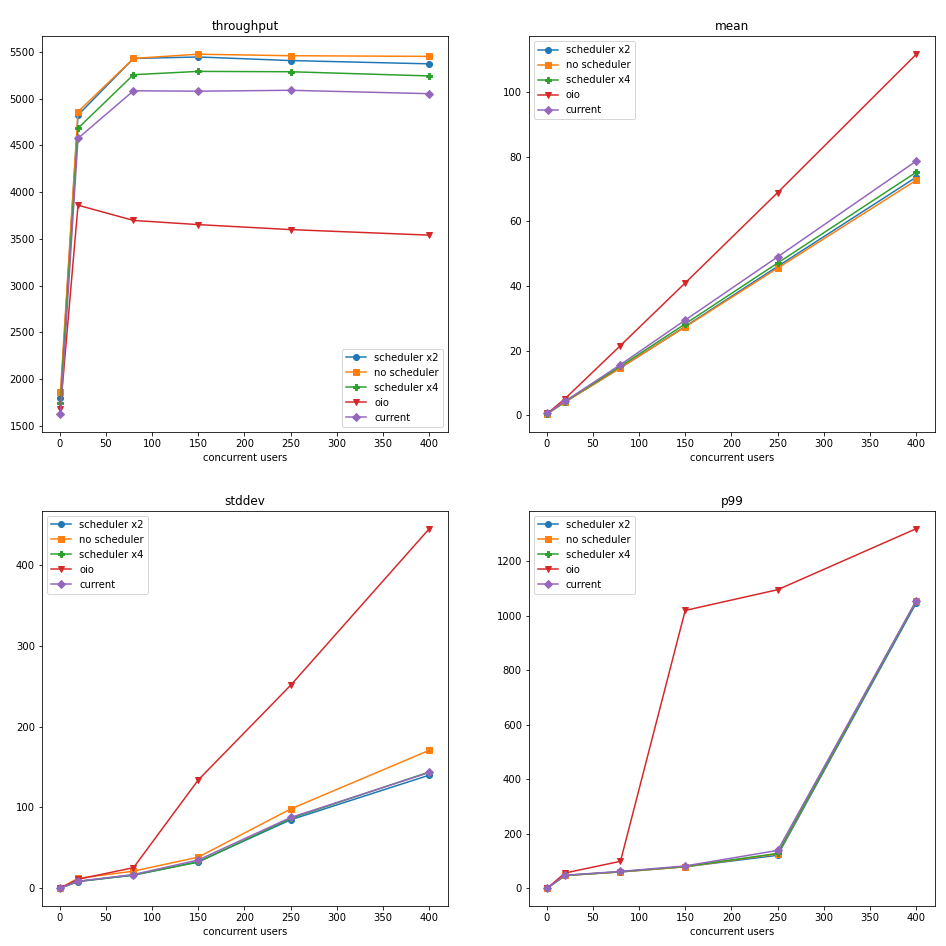
\includegraphics[scale=0.35]{figures/prime_small test results.png}
 	\end{center}
 	\caption{Sample experiment result}
 	\label{sample_result}
 \end{figure}

Then each metric is evaluated against each test program and each architectural change mentioned above.

\begin{comment}

\begin{table}[]
\begin{center}
\begin{tabular}{|l|l|l|l|l|l|}
\hline
Test case                                                     & \multicolumn{5}{l|}{Server architecture}                                                                                                                                                                                                                                \\ \hline
& \begin{tabular}[c]{@{}l@{}}Ballerina \\ original\end{tabular} & \begin{tabular}[c]{@{}l@{}}No \\ scheduler\end{tabular} & Netty OIO & \begin{tabular}[c]{@{}l@{}}Thread pool\\  size x 2\end{tabular} & \begin{tabular}[c]{@{}l@{}}Thread pool\\  size x 4\end{tabular} \\ \hline
\begin{tabular}[c]{@{}l@{}}Prime check \\ small\end{tabular}  &                                                               &                                                         &           &                                                                 &                                                                 \\ \hline
\begin{tabular}[c]{@{}l@{}}Prime check \\ medium\end{tabular} &                                                               &                                                         &           &                                                                 &                                                                 \\ \hline
\begin{tabular}[c]{@{}l@{}}Prime check \\ large\end{tabular}  &                                                               &                                                         &           &                                                                 &                                                                 \\ \hline
\begin{tabular}[c]{@{}l@{}}Database \\ call (IO)\end{tabular} &                                                               &                                                         &           &                                                                 &                                                                 \\ \hline
Merger sort                                                   &                                                               &                                                         &           &                                                                 &                                                                 \\ \hline
File read                                                     &                                                               &                                                         &           &                                                                 &                                                                 \\ \hline
\end{tabular}
\end{center}
\caption{Architecture comparison metric}
\label{tab:result_metric}
\end{table}

\end{comment}


Architectural changes to existing Ballerina run time involved extensive debugging because bugs in the implementation may incur wrong results. Therefore, this phase is conducted in an iterative manner to verify the results.
At the end of this stage, no architecture was performed well for IO use cases rather than CPU intensive cases and vice versa. Although changing thread pool size in the Ballerina scheduler started to show some significant results. Increasing thread pool size was affected differently in IO use cases. Then phase 2 is designed to analyze the variation of thread pool comprehensively.



\subsection{Phase II - Tuning thread pool size}

Thread pool tuning can be approached in two ways, \textbf{(1) White box system} — This requires complex mathematical modeling with queuing theories \cite{math_aproach_thread_pool_tuning}. Also, assumptions made at the beginning make it difficult to apply those modeling techniques for practical scenarios. \textbf{(2) Black box system} — In this approach, the thread pool system is considered as a black box where in-depth analysis of the thread pool system is not performed. Experiments are performed heuristically by changing parameters such as the size of the thread pool. Figure \ref{black_box_boundary} shows the boundary of the black box.
 
\begin{figure}[htbp]
	\begin{center}
		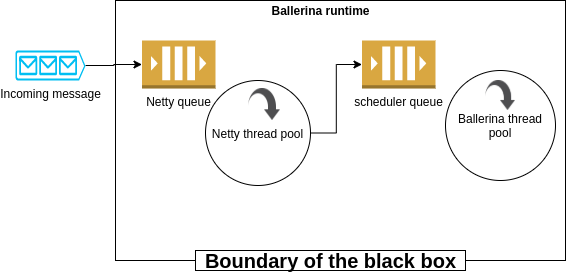
\includegraphics[scale=0.5]{figures/black_box_boundary.png}
	\end{center}
	\caption{Boundary of the black box}
	\label{black_box_boundary}
\end{figure}


This phase is preceded by considering the system as the black box. This model allows executing different programs under different sizes of the thread pool. Following the first phase of experiments, it is identified that changing thread pool size is affected differently for programs that consist of IO features. In the previous phase, experiments are conducted under different concurrency levels, but in this phase, fixed concurrency level is selected. Concurrency level was selected where a number near the point in the throughput curve which curve is starting to get flatten.

New sets of programs are implemented referring to multiple sources \cite{Ballerina_Performance,Ballerina_Website} in order to support programs that have rich IO call variations. In addition to the database calls in previous phase programs which have remote HTTP calls, GRPC calls and loops that contain these features are implemented. Subsection \ref{sub:phase3} provide more information. CPU intensive programs are no longer considered since it is difficult to extract CPU intensive operations directly by parsing AST. A more IO-oriented approach is used where the AST parser able to extract this information directly from the source code.  
	
\subsubsection{Experimental design} 

As a primary metric of evaluation average latency is used. Then each program is run under different thread pool sizes. Afterward, metrics are recorded. Table \ref{tab:pool_size_latency} shows summary of the results. Empty cells represent the average latency. Minimum latency values provide the optimal thread pool size for a given program. Instead of declaring thread pool size as a multiplier of the number of CPUs, explicit numbering is used for in-depth analysis of every thread pool size from 1 to 22. This range is selected because latency is always getting higher when increasing the number further.    

\begin{table}[]
	\caption{Program vs. Thread pool size - Latency results }
	\subcaption{The propose of this tabele is providing the insight of how data is gahtherd. Eplicit values are not presented here. Rsults section plots exact values }
	\begin{center}
	\begin{tabular}{|l|l|l|l|l|l|l|}
		\hline
		Program    & \multicolumn{6}{l|}{Pool size}        \\ \hline
		& 1            & 2 & 3 & ... & 19 & ... \\ \hline
		Program 1  & Ave. latency    & ...  & ...  & ...  &... &     \\ \hline
		Program 2  &      ...        & ...  & ...  & ...  &... &     \\ \hline
		Program 3  &      ...        & ...  & ...  & ...  &... &     \\ \hline
		...        &      ...        & ...  & ...  & ...  &... &     \\ \hline
		Program 50 &      ...        & ...  & ...  & ...  &... &     \\ \hline
		...        &      ...        & ...  & ...  & ...  &... &     \\ \hline
	\end{tabular}
	\end{center}
	\label{tab:pool_size_latency}
\end{table}

\subsection{Phase III - Building machine learning model to predict optimal thread pool size for given program}\label{sub:phase3}

At first, two models are considered in addition to predicting optimal thread pool. One model directly predicts the latency with given program features and given thread pool size. This model can be expressed as following function. 

$$ Latency \:(ms) = f(\:Program\:features,\:Threadpool\:size\:)$$

The weakness of this model is it heavily depends on the nature of the IO call. As an example latency is dependent on where the database is hosted if the given program has a database call. Also, latency is affected by the network connection also. Then the generalization of the result is very difficult.

The next model predicts optimal thread pool size for the given program. That model can be expressed as follows. That is the hypothesis that tries to resolve using a machine learning model. 

$$ Optimal\:thread\:pool\:size = f(\:Program\:features)$$

In order to build this model it is required find the minimum thread pool value from the result obtained by Design phase II. This step can be depicted as in figure \ref{optimal_pool_size}

\begin{figure}[htbp]
	\begin{center}
		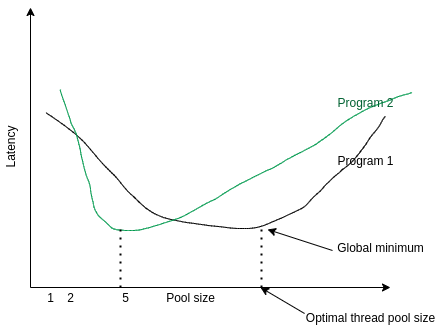
\includegraphics[scale=0.5]{figures/optimal_pool_size.png}
	\end{center}
	\caption{Obtaining optimal thread pool size}
	\label{optimal_pool_size}
\end{figure}

After some feature engineering steps, Features in table \ref{tab:programming-features}  are selected to train the machine learning model. Hyper parameters of each machine learning model are tuned for better accuracy. The implementation of hyper parameter tuning is presented in chapter \ref{chap:4}.

\begin{table}[]
	\caption{Programming features selected for machine learning model}
	\label{tab:programming-features}
	\begin{tabular}{|l|l|}
		\hline
		& Feature                                                      \\ \hline
		F1 & Number of HTTP connector calls                               \\ \hline
		F2 & Number of Database connector calls                           \\ \hline
		F3 & Number of non-blocking gRPC connector calls                  \\ \hline
		F4 & Number of loops containing HTTP connector calls              \\ \hline
		F5 & Number of loops containing Database connector calls          \\ \hline
		F6 & Number of loops containing non-blocking gRPC connector calls \\ \hline
	\end{tabular}
\end{table}

Then a training data set is created where input features are above programming features and output is optimal thread pool size. Table \ref{tab:data_frame} shows the shape of the data frame.


	\begin{table}[]
		\caption{Data frame shape of the training data set }
		\label{tab:data_frame}
		\begin{center}
		\begin{tabular}{|l|l|l|l|l|l|}
			\hline
			\multirow{2}{*}{Program} & \multicolumn{4}{l|}{Features} & \begin{tabular}[c]{@{}l@{}}Optimal Thread pool\\  size\end{tabular} \\ \cline{2-6} 
			& F 1    & F2    & ..    & Fn   &                                                             \\ \hline
			Program 1                &  ...  &  ...     &   ...    &  ...   &       n1                              \\ \hline
			...                      &  ...  &  ...     &   ...    &  ...   &       n2                              \\ \hline
		\end{tabular}
	\end{center}
		
	\end{table}

Then following machine learning models are selected and evaluated the accuracy of each model.

\begin{itemize}
	
	\item XGBoost
	\item Support Vector Machine
	\item Decision Tree
	\item Random Forest
	
\end{itemize}

For regression models \acrfull{MAPE} and \acrfull{MSE} are evaluated. For classification models F1 score and accuracy are evaluated.

The problem is originally a regression problem because the output of the model is a quantity (thread pool size). As this research provides a proof of concept, the problem is formulated as a classification model as well. Mapping the problem into a classification is possible because, as in the results of optimal thread pool sizes, clear clusters are visible. Chapter \ref{chap:5} provide results. Moreover, the distribution of the optimal thread pool is not uniform and only has several values.

\subsection{Phase IV - Parsing Ballerina AST to obtain features}\label{phase_iv}

First off, it is better to have some idea about what is \acrfull{AST}. It is a tree representation of the stricture of the source code.AST does not include all the details such as semicolon, parenthesis, etc. AST is used in semantic analysis of a code during the compilation process. Traversal of the AST verifies the correctness of the program against rules provided for that language. Moreover, information of the code can be extracted by traversing the AST.  Example of an AST is shown in figure \ref{AST_example} for code segment shown in figure \ref{code_for_ast}.

\begin{figure}[htbp]
	\begin{center}
		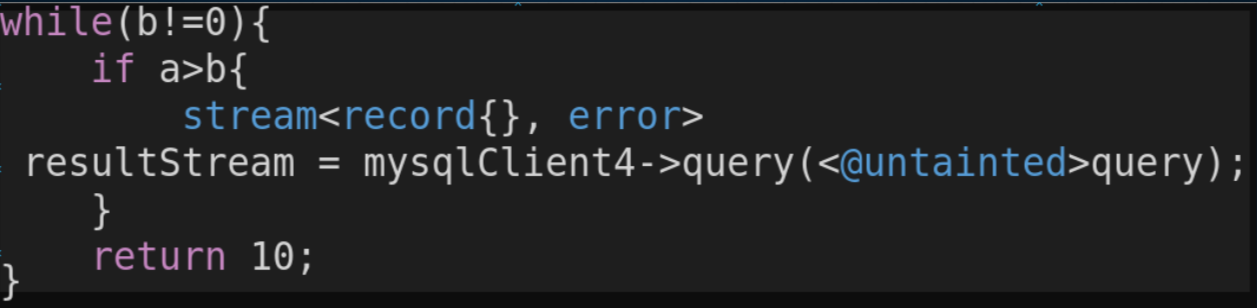
\includegraphics[scale=0.3]{figures/sample_code_for_ast.png}
	\end{center}
	\caption{Ballerina code}
	\label{code_for_ast}
\end{figure}

\begin{figure}[htbp]
	\begin{center}
		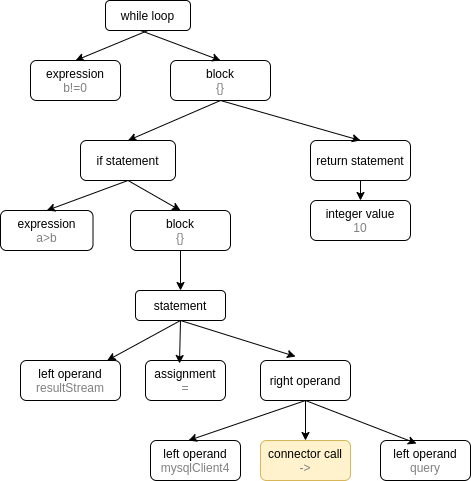
\includegraphics[scale=0.5]{figures/AST example.png}
	\end{center}
	\caption{Example AST}
	\label{AST_example}
\end{figure}

In this phase, a module is designed to parse Ballerina source code to feed the features into a machine learning model. Manual feature extraction is erroneous and harder when programs are large. First, this module accepts the Ballerina source code and output the array of features which is fed to the machine learning model. This is where Ballerina specific features are used that other languages are lack. 
Services are first-order functions in the Ballerina language. Then it is able to decide that the given program contains a web service. Then the subsequent parsing happens inside these service definitions. Also, network calls are part of the language. In the other languages, they are mostly library calls which is difficult to identify the given line of code that contains a network call. In Ballerina this is called a connector call. Recalling section \ref{Sec_Ballerina}, other languages provide network operations as library functions. If we try to extract such features from other languages, we need to know exactly which function call does an IO operation. In Ballerina, it is possible because connector calls can be differentiated naively. Algorithm 1 is implemented to extract features.

\begin{algorithm} \label{alg:ast_parser}
	
	\SetAlgoLined
	\KwIn{Source code (Ballerina.toml) }
	\KwOut{Feature Array}
	Start parsing\;
	
	\While{End program}{
		
		Traverse node\;{
			\If{Right Arrow Found}{
				
				\If{Left operand is Kind(Database call)}
				{
					\While{Backtrack}{
						
						\If{Loop start found}{
							Update feature array (Database call inside loop + 1)\;
							Stop backtracking and continue parsing\;
						}
						
						Update feature array (Direct Database call + 1)\;
						Continue parsing\;
					}
					
				}
			
				\If{left operand is Kind(Http call)}
				{
					\While{Backtrack}{
						
						\If{Loop start found}{
							Update feature array (HTTP call inside loop + 1)\;
							Stop backtracking and continue parsing\;
						}
						
						Update feature array (Direct HTTP call + 1)\;
						Continue parsing\;
					}
					
				}
			
				\If{left operand is Kind(GRPC-non-blocking call)}
				{
					\While{Backtrack}{
						
						\If{Loop start found}{
							Update feature array (GRPC call inside loop + 1)\;
							Stop backtracking and continue parsing\;
						}
						
						Update feature array (Direct GRPC call + 1)\;
						Continue parsing\;
					}
					
				}
				
			}
		}
		
			
	}
	
	\caption{Extract features using Ballerina AST}
\end{algorithm}

\section{Final design}\label{sec:final_design}

Finally, combing the above design steps, the overall design of the research is shown in figure \ref{hl_architecture}. First off, the Model is trained by different program features. In the second step trained machine learning model is produced. Then the model is given a new Ballerina source file. Program features are automatically extracted by AST parser. Then model output the optimal thread pool size for that given program. Then the program can be compiled with the suggested thread pool size. 

\section{Limitations}

There are several limitations that can be reorganized in the design. In design phase II, a fixed concurrency level is chosen. It is not explored how different concurrency levels are affected to the results. Another limitation is that hardware variable such as the number of CPUs, memory are not considered when constructing the hypothesis. Finally, when constructing the machine learning model it is only considered IO features. CPU extensive programs cannot be identified by parsing the source code. More explanations of these limitations are presented in chapter \ref{chap:6}.

